
\begin{center} 
\emph{``The people who oppose your ideas are inevitably those who represent the established order that your ideas will upset.'' -- Anthony J. D'Angelo}
\end{center}

\section{Representations of Linear Transformations as Matrices}\label{sec:representation}
We have seen before that linear transformations are those maps between vector spaces which preserve the vector structure, that is, preserve vector addition and scalar multiplication. We have seen that matrix multiplication is a linear transformation, hence all the geometric transformations in the previous section are linear transformations. We will now see that all linear transformations are essentially just matrix multiplication. \\

\begin{Exam}
Let $\bb e_1 = \vr{1\\0}$ and $\bb e_2 = \vr{0\\1}$. Suppose that $T : \R^2 \to \R^3$ is a linear transformation such that \[T(\bb e_1) = \vr{1\\2\\3}\qquad\text{and}\qquad T(\bb e_2) = \vr{3\\-5\\0}.\] With no additional information, find a formula for the image of an arbitrary vector $\bb x \in \R^2$.\\

Since $\bb x = \vr{x_1 \\ x_2} = x_1\bb e_1 + x_2\bb e_2$ and since $T$ is a linear transformation, it must hold that 
\begin{eqnarray*}
T(\bb x) &=& T(x_1\bb e_1 + x_2\bb e_2) = x_1T(\bb e_1) + x_2T(\bb e_2)\\
&=& x_1\vr{1\\2\\3} + x_2\vr{3\\-5\\0} = \mtx{c}{x_1+3x_2\\ 2x_1-5x_2 \\ 3x_1} = \mtx{rr}{1&3\\2&-5\\3&0}\bb x.
\end{eqnarray*} In particular, $T$ can be represented as a matrix transformation.
\end{Exam}\vs

The argument applied in the previous example works in general. \\

\begin{Thm} Let $\bb e_i$ be the vector in $F^n$ such that the $i$th entry is 1 and all other entries are 0. Let $T : F^n \to F^m$ be a linear transformation and let $A = \mtx{rrrrr}{T(\bb e_1) & T(\bb e_2) & \ldots & T(\bb e_n)}$. Let $\bb x \in F^n$. Then 
\[T(\bb x) = A\bb x.\] This matrix $A$ is called the \textbf{standard matrix for the linear transformation} $T$ and is often denoted $[T]$.
\end{Thm}\vs

\begin{Exam} Find the standard matrix $A$ for the linear transformation $T(x_1,\ x_2) = (3x_1+x_2,\ 2x_1-4x_2)$.\\

Since $T(\bb e_1) = (3,\ 2)$ and $T(\bb e_2) = (1,\ -4)$, we have that $[T] = A = \mtx{rr}{3&1\\2&-4}$ and \[T(\bb x) = A\bb x =  \mtx{rr}{3&1\\2&-4}\bb x.\qedhere\]
\end{Exam}\vs

Recall that if $S : F^m\to F^p$ and $T : F^n \to F^m$ are functions, then their composite $S\circ T$ is the function given by the rule $(S\circ T)(\bb x) = S(T(\bb x))$ where $\bb x\in F^n$. Functions are often viewed, by parable, as machines on a conveyor belt. As an element $\bb x$ in the domain of $T$ rolls into the machine $T$, it is transformed into the element $T(\bb x)$. The composite $S\circ T$ is then the machine formed by placing the machines $S$ and $T$ next each other on the conveyor belt. The following theorem states that matrix representations are compatible with function composition.

\centerline{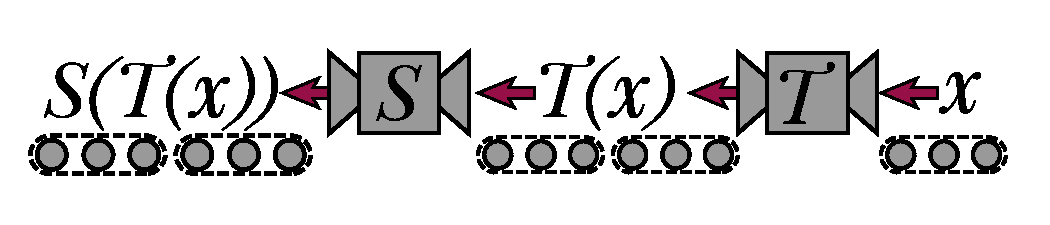
\includegraphics[scale=1]{Chapter3/images/SoT.pdf}}
%{\vspace{-10 pt}\hfill\footnotesize (Image contributed by Maria Langford)}\\ %Plagiarized?

\begin{Thm} Let $S : F^m\to F^p$ and $T : F^n \to F^m$ be linear transformations with standard matrices $A$ and $B$, respectively. Let $\bb x \in F^n$. Then 
\[S\circ T(\bb x) = S(T(\bb x)) = AB\bb x,\] that is, the matrix which represents the composite of two linear transformations is the product of their matrix representations.
\end{Thm}\vs

Recall that a linear transformation $T : F^n\to F^m$ is \emph{one-to-one} if and only if $T(\bb x) = T(\bb y)$ implies that $\bb x=\bb y$ if and only if $\ker T = \{\bb 0\}$, that is, the only vector mapping to zero is zero itself. Given the matrix representation $[T] = A$, we see that $\ker T = \null A$, that is, the vectors mapped to $\bb 0$ by $T$ are exactly those vectors whose product with $A$ is $\bb 0$. Hence, finding the null space of $A$ is equivalent to finding the kernel of $T$. In particular, a linear transformation is one-to-one if and only if the columns of its matrix representation are linearly independent.\\

\begin{Exam}\label{exam:transT} Let $T : \R^2 \to \R^3$ be a transformation given by the rule
\[T(x,y) = (x+y, 0, 2x+3y).\] Then 
\[[T] = \mtx{cc}{T(\bb e_1) & T(\bb e_2)} = \mtx{rr}{1&1\\0&0\\2&3} \sim \mtx{rr}{1&1\\2&3\\0&0} \sim \mtx{rr}{1&2\\0&1\\0&0} \sim \mtx{cc}{\fbox{$1$}&0\\0&\fbox{$1$}\\0&0}.\] The row-reduced echelon form of $[T]$ shows that the columns of $[T]$ are linear independent since there is  a pivot in each column. Therefore, $T$ is one-to-one, that is, $\ker T=\{\bb 0\}$.
\end{Exam}\vs

\begin{Exam}\label{exam:transS} Let $S : \R^3 \to \R^2$ be a linear transformation given by the rule 
\[S(x, y, z) = (x+y-2z, -y+z).\] Then 
\[[S] = \mtx{ccc}{S(\bb e_1) & S(\bb e_2) & S(\bb e_3)} = \mtx{rrr}{1&1&-2\\0&-1&1} \sim \mtx{rrr}{1&1&-2\\0&1&-1} \sim \mtx{ccr}{\fbox{$1$}&0&-1\\0&\fbox{$1$}&-1}.\] The row-reduced echelon form of $[S]$ shows that the columns of $[S]$ are linear dependent since there is no pivot in the third column. Therefore, $S$ is not one-to-one. In particular, $\ker S= \Span\{[1, 1, 1]^\top \}$.
\end{Exam}\vs

The homogeneous system $A\bb x = \bb 0$ has a nontrivial solution when $A$ has a non-pivot column. The nullity of $A$ is the number of non-pivot columns in $A$. If $A$ is an $m\times n$ matrix and $m<n$, that is, $A$ has more columns than rows, then $A$ necessarily has non-pivot columns. Hence, the $\text{nullity}(A) \ge 1$.\\

Recall that a linear transformation $T: F^n\to F^m$ is \emph{onto} if and only if for all vectors $\bb b\in F^m$ there exists a vector $\bb x\in F^n$ such that $T(\bb x) = \bb b$ if and only if $\im(T) = F^m$, that is, the set of images of $T$ is the whole target space $F^m$. Given the matrix representation $[T] = A$, we see that $\im  T = \col A$, that is, the vectors which are linear combinations of the columns of $A$ are exactly the vectors which can come out of $T$. Hence, finding the column space of $A$ is equivalent to finding the image of $T$. In particular, a linear transformation is onto if and only if the columns of its matrix representation span $F^m$.\\

\begin{Exam} Let $T : \R^2 \to \R^3$ be the transformation given in \examref{exam:transT}. The row-reduced echelon form of $[T]$ shows that $[T]$ has no pivot in the third row. Therefore, $T$ is not onto. In particular, $[0, 1, 0]^\top \notin \im T$.
\end{Exam}\vs

\begin{Exam} Let $S : \R^3 \to \R^2$ be the transformation given in \examref{exam:transS}. The row-reduced echelon form of $[S]$ shows that $[S]$ has a pivot in each row. Therefore, $S$ is onto. In particular, $\im S = \R^2$.
\end{Exam}\vs

The inconsistency of the equation $A\bb x=\bb b$ may occur when $A$ has a row of zeros in echelon form but the corresponding position in the augmented column is nonzero. In this case, consistency is dependent on the choice of $\bb b$ and at least one choice of $\bb b$ will make $A\bb x= \bb b$ inconsistent. These rows of zeros in the echelon form correspond to non-pivot rows of $A$. Let the \textbf{conullity} of $A$ denote the number of non-pivot rows of $A$.  If $A$ is an $m\times n$ matrix and $m>n$, that is, $A$ has more rows than columns, then $A$ necessarily has non-pivot rows. Hence, the $\text{conullity}(A) \ge 1$.\\

\begin{Prop} Let $T : F^n\to F^m$ is a linear transformation. 
\begin{enumerate}[!THM!]
\item If $m>n$, that is, $[T]$ has more rows than columns, then $T$ cannot be onto.
\item If $m<n$, that is, $[T]$ has more columns than rows, then $T$ cannot be one-to-one.
\end{enumerate}
\end{Prop}\vs

%%Every vector space can be expressed in coordinates making it essentially the same thing as $\R^n$. We say that $V$ and $\R^n$ are \textbf{isomorphic}, denoted $V\cong \R^n$, meaning that although the two spaces are different in their appearance and essentially the same shape. More precisely, an \textbf{isomorphism} is a bijective linear transformation. Such a mapping produces a one-to-one correspondence between vectors of the two spaces that preserves the algebraic structure. For example, the function $T : \P_n \to \R^{n+1}$ given by the rule
%%\[a_0 + a_1t + a_2t^2 + \ldots + a_nt^n \quad\longmapsto\quad \vr{a_0\\a_1\\a_2\\\vdots\\a_n}\] is an isomorphism. This means that $\P_n$ and $\R_{n+1}$ are essentially the same vector space.\\

%Let $V$ and $W$ be $n$- and $m$-dimensional vector spaces with bases $\B = \{\bb b_1, \ldots, \bb b_n\}$ and $\C = \{\bb c_1, \ldots, \bb c_m\}$, respectively. Let $T: V\to W$ be a linear transformation. Likewise, the coordinate mappings $[\cdot]_\B : V \to \R^n$ and $[\cdot]_\C : W \to \R^m$ are linear transformations (in fact, they are isomorphisms). Consider the composite linear transformation $([\cdot]_\C\circ T\circ [\cdot]_\B^{-1}) : \R^n\to \R^m$. This is a linear transformation between $\R^n$ and $\R^m$. Let $A$ be the standard matrix of this composite transformation. Then 
%\[[T(\bb x)]_\C = A[\bb x]_\B\] for all $\bb x\in V$. This matrix $A=  \,_\C[T]_\B$ is called the \textbf{standard matrix} of $T$ relative to $\B$ and $\C$. In fact, 
%\[A = \mtx{cccc}{[T(\bb b_1)]_\C & [T(\bb b_2)]_\C & \ldots & [T(\bb b_n)]_\C}.\] The matrix $\,_\C[T]_\B$ is sometimes called a \textbf{matrix representation} of the linear transformation $T$. The following diagram may be useful in remembering the relationship here:
%\begin{center}
%\begin{tikzpicture}
%\path (0,0) node (x) {$\bb x$};
%\path (x) ++ (3,0) node (Tx) {$T(\bb x)$};
%\path (x) ++ (0,-1.5) node (xB) {$[\bb x]_\B$};
%\path (xB) ++ (3,0) node (TxC) {$[T(\bb x)]_\c$};
%\draw[thick, ->] (x) -- (Tx) node[midway, above] {$T$};
%\draw[thick, ->] (xB) -- (TxC) node[midway, above] {$A$};
%\draw[thick, ->]  (x) -- (xB);
%\draw[thick, ->]  (Tx) -- (TxC);
%\end{tikzpicture}
%\end{center}
%
%\begin{Exam}Suppose $\B = \{\bb b_1, \bb b_2\}$ is a basis for $V$ and $\C = \{\bb c_1, \bb c_2, \bb c_3\}$ is a basis for $W$. Let $T : V\to W$ be a linear transformation such that 
%\[T(\bb b_1) = 3\bb c_1 - 2\bb c_2 + 5\bb c_3\qquad T(\bb b_2) = 4\bb c_1 + 7\bb c_2 - \bb c_3.\] Then 
%\[[T(\bb b_1)]_\C =  \vr{3\\-2\\5}\qquad\text{and}\qquad [T(\bb b_2)]_\C =  \vr{4\\7\\-1}.\] This gives
%
%\[A = \mtx{cc}{[T(\bb b_1)]_\C & [T(\bb b_2)]_\C} =\mtx{rr}{3&4\\-2&7\\5&-1}.\qedhere\]
%\end{Exam}\vs
%
%When $T : V \to V$ is a linear transformation with the same domain and codomain, we often use the same basis for the domain and codomain. \\

%%\begin{Exam} The mapping $D : \P_2 \to \P_2$, defined by 
%%\[D(a_0+a_1t+a_2t^2) = a_1+2a_2t,\] is linear (this is just the derivative). \\
%%\begin{enumerate}[(a)]
%%\begin{multicols}{2}
%%\item Find the standard matrix of $D$ relative to $\B$, where $\B = \{1, t,t^2\}$.\\
%%
%%Since $D(1) = 0$, $D(t) = 1$, and $D(t^2) = 2t$, we have that:  \columnbreak
%%\[[D]_\B = \mtx{rrr}{0&1&0\\0&0&2\\0&0&0}.\]
%%\end{multicols}\vs
%%
%%\item Verify that $[D(\bb p)]_\B = [D]_\B[\bb p]_\B$ for all $\bb p\in \P_2$.\\
%%
%%Let $\bb p(t) = a_0+a_1t+a_2t^2$. Then  $[\bb p]_\B = \vr{a_0\\a_1\\a_2}$ and $[D]_\B[\bb p]_\B = \mtx{rrr}{0&1&0\\0&0&2\\0&0&0}\vr{a_0\\a_1\\a_2} = \vr{a_1\\2a_2\\ 0}.$ On the other hand, $[D(\bb p(t)]_\B = [a_1+2a_2t]_\B = \vr{a_1\\2a_2\\0}.$ Therefore, the two forms agree. \hfill$\qedhere$
%%\end{enumerate}
%%\end{Exam}
%
%%Let $\B = \{\bb v_1, \ldots, \bb v_n\}$ be a basis for a vector space $V$. Let $\bb x, \bb y\in V$ such that 
%%\[\bb x= c_1\bb v_1 + \ldots + c_n\bb v_n\quad\text{and}\quad \bb y= d_1\bb v_1 + \ldots + d_n\bb v_n.\] Then
%%\[[\bb x]_\B = \mtx{c}{c_1\\\vdots\\c_n}\quad\text{and}\quad[\bb y]_\B = \mtx{c}{d_1\\\vdots\\d_n}.\] Thus, 
%%\[[\bb x + \bb y]_\B = [(c_1+d_1)\bb v_1+\ldots + (c_n+d_n)\bb v_n]_\B = \mtx{c}{c_1+d_1\\\vdots\\c_n+d_n} = \mtx{c}{c_1\\\vdots\\c_n} + \mtx{c}{d_1\\\vdots\\d_n} = [\bb x]_\B + [\bb y]_\B.\] Likewise, for any $r\in \R$, 
%%\[[r\bb x]_\B = [rc_1\bb v_1 + \ldots + rc_n\bb v_n]_\B =  \mtx{c}{rc_1\\\vdots\\rc_n} = r\mtx{c}{c_1\\\vdots\\c_n} = r[\bb x]_\B.\] Therefore, the change-of-coordinates map $[\cdot]_\B : V \to \R^n$ is a linear transformation. In fact, it is even bijective (it maps a basis onto a basis). 
%%
%%\begin{Thm}[Theorem 8] Let $\B = \{\bb b_1, \ldots, \bb b_n\}$ be a basis for a vector space $V$. Then the coordinate mapping $\bb x \mapsto [\bb x]_\B$ is an isomorphism, that is, a bijective linear transformation.
%%\end{Thm}\vs
%%
%%Of special interest is the case when $V = \R^n$, because we can then compute the standard matrix of $[\cdot]_\B$. Let the \textbf{change-of-coordinates matrix} 
%%\[P_\B = \mtx{cccc}{\bb b_1 & \bb b_2 & \ldots & \bb b_n}\] be defined. Then 
%%\[\bb x = P_\B[\bb x]_\B\] for all $\bb x\in \R^n$, and \[P_\B^{-1}\bb x = [\bb x]_\B.\]\vs
%
%%\begin{Def} Suppose the set $\B = \{\bb v_1, \bb v_2, \ldots, \bb v_n\}$ is a basis for a vector space $V$. For each $\bb x\in V$, the \textbf{coordinates of $\bb x$ relative to the basis $\B$} are the weights $c_1, \ldots, c_n$ such that 
%%\[\bb x = c_1\bb v_1 + c_2\bb v_2 +\ldots + c_n\bb v_n.\] The vector in $\R^n$
%%\[[\bb x]_\B = \mtx{c}{c_1\\\vdots\\c_n}\] is called the \textbf{coordinate vector of $\bb x$ relative to $\B$} or the \textbf{$\B$-coordinate vector of $\bb x$}.
%%\end{Def}\vs 
%
%%So even in abstract settings, linear transformations are nothing more than just matrices. In fact, the kernel of a linear transformation in coordinates is just the null space of its matrix representation. Likewise, the range of the transformation in coordinates just the column space of the matrix representation. As we have seen before with matrix transformations $T : \bb x \mapsto A\bb x$ for an $m\times n$ matrix $A$, the columns of $A$ span $\R^m$ if and only if $T$ is onto and the columns of $A$ are linearly independent if and only if $T$ is one-to-one. Combining this with the Basis Theorem, which says that if a spanning set or linearly independent set have the same size as the dimension then it is a basis, we get more conditions equivalent to nonsingularity.
%%

%%%%%%%%%%%%%%%%%% Exercises %%%%%%%%%%%%%%%%%%%
\startExercises{representation}

\noindent For Exercises \ref{exer:standardmatrixstart}-\ref{exer:standardmatrixstop}, for the linear transformations $T$ find its standard matrix $[T]$.%NEW
\begin{enumerate}[!HW!, start=1, label=$\spadesuit$ \arabic*., ref=\arabic*]
\item\label{exer:standardmatrixstart} $T : \R^2\to \R^2 : T(x_1,x_2) = (2x_1-x_2, -4x_2)$.
\itemspade $T : \R^3\to \R^4 : T\left(\vr{x_1\\x_2\\x_3}\right) = \mtx{c}{x_1+2x_2+x_3\\ 3x_1+14x_3-5x_2 \\  3x_2 - 5x_1-18x_3 \\ 19x_2-7x_1-40x_3}$.
\itemspade $T : \C \to \C^4 : T(z) = (z, iz, -z, -iz)$.
\itemspade $T : \Z_2^4 \to \Z_2 : T(x_1, x_2, x_3, x_4) = x_1+x_2+x_3+x_4$.
\item\label{exer:standardmatrixstop}  $T : \Z_5^3\to \Z_5^3 : T(x_1,x_2,x_3) = (x_3, x_2, x_1)$.
\end{enumerate}

\noindent For Exercises \ref{exer:standardmatrixcompositestart}-\ref{exer:standardmatrixcompositestop}, find the standard matrix of the composite function $S\circ T$. %NEW
\begin{enumerate}[!HW!, label=$\spadesuit$ \arabic*., ref=\arabic*]
\item\label{exer:standardmatrixcompositestart}\label{exer:standardmatrixcompositestop}
$T : \R^2 \to \R^3 : T(x_1,x_2) = (2x_2, 3x_1, 2x_1-3x_2)$ and $S : \R^3\to \R^2 : S(y_1, y_2, y_3) = (y_3-2y_2, y_1-2y_3)$
\end{enumerate}

\noindent For Exercises \ref{exer:standardmatrixnullstart}-\ref{exer:standardmatrixnullstop}, determine if the given linear transformation from Exercises \ref{exer:standardmatrixstart}-\ref{exer:standardmatrixstop} is one-to-one or onto. Find a basis for its kernel and for its image.%NEW
\begin{enumerate}[!HW!, label=$\spadesuit$ \arabic*., ref=\arabic*]
\begin{multicols}{5}
\item\label{exer:standardmatrixnullstart}
Exercise \ref{exer:standardmatrixstart}
\itemspade \FPeval{\result}{clip(\getrefnumber{exer:standardmatrixstart}+1)} Exercise \result
\itemspade \FPeval{\result}{clip(\getrefnumber{exer:standardmatrixstart}+2)} Exercise \result
\itemspade \FPeval{\result}{clip(\getrefnumber{exer:standardmatrixstart}+3)} Exercise \result
\item\label{exer:standardmatrixnullstop}  Exercise \ref{exer:standardmatrixstop}\
\end{multicols}
\end{enumerate}

\noindent QUICK! For Exercises \ref{exer:standardmatrixnullstart}-\ref{exer:standardmatrixnullstop}, determine in less than 10 seconds if the linear transformation CANNOT be one-to-one and if it CANNOT be onto. 
\begin{enumerate}[!HW!]
\item $T : \R^3\to \R^3 : T(x,y,z)=(x,y,z)$ %Jacob Kuhn
\item $T: \R^3\to \R^2 : T(x_1,x_2,x_3)=(x_1+2x_2, x_3-3x_2)$ %Daven Triplett
\item $T: \R^3\to \R^4 : T(x_1,x_2,x_3)=(2x_1+3x_3, x_2+4x_1+x_3, x_3+x_1+x_2, x_1+3x_2+x_3)$ %Daven Triplett
\item $T: \C \to \C^3 : T(z) = (z,z,z)$%Jacob Kuhn
\item $T:\C\to \C^3 : T(z) = ((3-i)z, (-2+2i)z, z)$ %Daven Triplett
\item $T: \Z_5^3 \to \Z_5 : T(x,y,z) = x+y+z$%Jacob Kuhn
\item $T: \Z_7^2\to \Z_7^2 : T(x,y)=(4x+2y, 3y)$ %Daven Triplett
\end{enumerate}

%%%%%%%%%%%%%%%%%%% Footnotes %%%%%%%%%%%%%%%%%%%
 %\mbox{}\vfill